\begin{section}{Materials and Methods}

All chemicals were purchased from Sigma-Aldrich and used without further purification, except: tetrahydrofuran and diethyl ether used in the syntheses were distilled on potassium and benzophenone under nitrogen atmosphere; B-(5'-formyl[2,2'-bi\-thio\-phen]\-5-yl)\-boronic acid was purchased from Tokyo Chemical Industry (\textsmaller{TCI}) and purified on a \SI{3}{\cm} silica gel column washing with dichloromethane and recovering with ethyl acetate; scalemic 2-methyl-1-butanol was purchased from Merck-Schuchardt and distilled under reduced pressure prior use.

All manipulations involving air-sensitive reagents or dry solvents were performed under an atmosphere of dry, filtered nitrogen. 

Thin layer chromatographies were performed using glass supported silica gel.

For flash chromatographies silica gel Merck 60 (0.04-\SI{0.06}{\mm}, flash) was used.

De\-oxy\-gen\-ated sodium carbonate aqueous solution was prepared by bubbling nitrogen in distilled water and after that sodium carbonate was added to obtain a \SI{1}{\Molar} solution.

Degassed ortho-di\-chloro\-benzene was bubbled with nitrogen and passed through three freeze-pump-thaw cycles.

Glassware used for reactions in nitrogen atmosphere were passed through three cycles of vacuum by mechanical pump, heating with heating gun and filling with nitrogen.

Common impurities found in tetra\-chloro\-ethane-d$_2$ used in \gls{NMR} analysis: {\HNMR} $\delta$ (ppm) 0.03 (s), 1.20 (s), 2.10 (s), 3.64 (dd), 5.14 (q); {\CNMR} $\delta$ (ppm) 29.62, 73.80 (t, solvent peak), 74.06 (s, solvent peak), 120.20. 

\ch{KCl} disks for \gls{UVvis} and \gls{CD} analysis were prepared grinding the solid in a mortar and consolidated with a press. 

Samples for photoluminescence measurements were prepared diluting with adequate amounts of methanol and chloroform a concentrated solution of the desired polymer in chloroform. After \SI{20}{\minute} samples were analyzed using in a glass cuvette. Some samples were measured again after further \SI{40}{\minute}.

\end{section}
\begin{section}{Instrumentation}

\Acrfull{FTIR} spectra were recorded using a \emph{Bruker \gls{FTIR} Tensor 27} spectrometer, samples were prepared as thin films cast on \ch{KBr} disk. Abbreviations used in reported spectra are: symm.\ (symmetrical), antisymm.\ (antisymmetrical), deform.\ (deformation), degen.\ (degenerate), arom.\ (aromatic).

Ultraviolet--visible (\gls{UVvis} ) spectra were recorded using using \emph{Jasco V-650} spectrophotometer and \SI{1}{\mm} path length quartz cuvette.

\label{fitting}
\Acrfull{CD} spectra were recorded using \emph{Jasco J-710} and a spectral window from \SI{230}{\nm} to \SI{600}{\nm}. Each measurement is repeated at least four times and a mean is reported. For measurements on films or solid a mean between various orientations of the substrate was reported, this helped to reduce artifacts from linear dichroism. Measurements on solutions were recorded using a \SI{1}{\mm} path length quartz cuvette. For estimating bisignate \gls{CD} peaks' center and amplitude the peaks were fitted with a sine waveform ($\mathrm{CD}= A+Bsin(C(\mathrm{wavelength}-D))$) using the Gnuplot software and considering only data points between 400 and \SI{500}{\nm}.

Spectra from \acrfull{GCMS} were recorded using GC \emph{Agilent 7890A} combined with detector 
\emph{Agilent 5975C MSD} and electron ionization source.

\Acrfull{DSC} analysis were accomplished using a \emph{Perkin Elmer Differential Scanning Calorimeter Pyris 1} instrument in absence of oxy\-gen. Heating rate: \SI{20}{\celsius\per\minute}, cooling rate: \SI{10}{\celsius\per\minute}.

\Acrfull{PL} spectra were collected with a setup consisting of \emph{Osram XBO} \SI{450}{\W} xenon lamp followed by a \emph{Jobin Yvon Horiba Gemini 180} monochromator, used for excitation wavelength selection, and a \emph{Spex 270M} monochromator combined with CCD, employed as a detector. The spectra were corrected for the instrument response functions. 

\Acrfull{NMR} spectra were collected at room temperature in 1,2-di\-deutero-1,1,2,2-tetra\-chloro\-ethane (\gls{TCE}-d2) and deuterated chloroform (\ch{CDCl3}) at the \gls{NMR} facility in ISMAC-CNR, Milan. All chemical shifts are reported in the standard $\delta$ notation of parts per million (ppm) using the peak of residual proton and carbon signals of \ch{CDCl3} ($\delta _{^1\mathrm{H}} = 7.26$, $\delta_{^{13}\mathrm{C}}=77.16$) and \gls{TCE}-d2 ($\delta _{^{1}\mathrm{H}}=5.94$, $\delta _{^{13}\mathrm{C}}=73.80$) as internal reference.

\Acrfull{SEC} measurements in Milan were performed using a \emph{GPCV 2000} pump and polystyrene standards. For measurements in chloroform at \SI{35}{\celsius} two columns \emph{PLgel Mixed C} (\SI{5}{\um} particle size) \emph{Polymer Laboratories} were used with a flux of \SI{0.8}{\mL\per\minute} and an injection volume of \SI{218.5}{\uL}. Two detectors were used: a \gls{UVvis} photo\-diode array \emph{DRI996} and a differential refractive index detector \emph{DRI2414}. 
For measurements in ortho-di\-chloro\-benzene at \SI{145}{\celsius} three columns \emph{PLgel Olexis Polymer Laboratories} were used with a flux of \SI{0.8}{\mL\per\minute} and an injection volume of \SI{218.5}{\uL}. Two detectors were used: a differential viscometer and a differential refractive index detector \emph{DRI2414}.

In \gls{SEC} measurements in Catania as a first step, relative averages ($M_n$, $M_w$, $M_z$) and polydispersity index (PDI = $M_w/M_n$) of all polymers were determined by a conventional size exclusion chromatography system calibrated toward polystyrene standards, using tetrahydrofuran as mobile phase, \SI{0.8}{\mL\per\minute} of flow rate and a temperature of \SI{35}{\celsius}. The conventional chromatographic system consisted of an integrated \emph{Alliance 2695} chromatographic system (de\-gasser, pump and injector) from \emph{Waters} (Milford, MA, USA) and a 2414 differential refractometer (DRI) used as concentration detector. The column set was composed of two PLgel Mixed C columns (\SI{5}{\um} of particle size) from \emph{Polymer Laboratories} (Shropshire, UK).

\Acrfull{MALDI} were recorded in the Institute of Chemistry and Technology of Polymers (\textsmaller{ICTP-CNR}, Catania) in reflector or linear delayed extraction mode, using a \emph{Voyager-DE STR} instrument (\emph{Perseptive Biosystem}) mass spectrometer, equipped with a nitrogen laser ($\lambda =$ \SI{337}{\nm}, pulse width = \SI{3}{\ns}), working in a positive ion mode. The accelerating voltage was \SI{20}{\kV}, grid voltage and delay time (delayed extraction, time lag), were optimized for each sample to achieve the higher mass resolution ($M / \Delta M$). Laser irradiance was maintained slightly above threshold. $\alpha$-Cyano-4-hydr\-oxy\-cinnamic acid and 1,8-di\-hydr\-oxy-9,10-di\-hydro\-anthracen-9-one (di\-thranol) \SI{0.1}{\Molar} in \gls{THF} were used as matrices. Then \SI{1}{\mL} of each analyte/matrix mixture was spotted on the \textsmaller{MALDI} sample holder and slowly dried to allow analyte/matrix co-crystallization. 

In \gls{SEC}\-/\gls{MALDI} combined analysis \SI{1}{\mL} fractions of each selected concentrated \gls{SEC} solutions was mixed with \SI{1}{\mL} or \SI{3}{\mL} of the matrix solution (trans-2-[3-(4-tert-butyl\-phenyl)-2-methyl-2-propenylidene]\-malononitrile, \textsmaller{DCTB}). Then, the same procedure used for the \gls{MALDI} analyses of the poly\-disperse polythiophene sample was followed. 

The \acrlong{WAXD} (\gls{WAXD} or \gls{XRD}) data were obtained at \SI{25}{\celsius} using a \emph{Siemens D-500} diffracto\-meter equipped with a \emph{Siemens FK 60-10} \SI{2000}{\W} tube (Cu K$_a$ radiation, $\lambda =$ \SI{0.154}{\nm}). 
The operating voltage and current were \SI{40}{\kV} and \SI{40}{\mA}, respectively. The data were collected from $2\theta =$ \SI{3}{\degree} to \SI{30}{\degree} at \SI{0.05}{\degree} intervals. 
\Acrfull{SAXS} measurements were conducted at \SI{25}{\celsius} with a \emph{Kratky Compact Camera}. Mono\-chromatized \ch{Cu} K$_a$ radiation 
($\lambda =$ \SI{0.154}{\nm}) was supplied by a stabilized \emph{Siemens Krystalloflex 710} generator and a \emph{Siemens FK 60-04}, \SI{1500}{\W} \ch{Cu} target tube operated at \SI{40}{\kV} and \SI{30}{\mA}.

\Acrfull{XRD2D} spectrum was recorded at \emph{Electra - Sincrotrone Trieste} synchrotron radiation facility in Trieste.

Spin coating were performed using \emph{Electron mec PRS 5V} spinner.

Annealing was performed using \emph{Mettler FP5} melting point apparatus.

Tests in solar cells were performed in Centre for Hybrid and Organic Solar Energy (\textsmaller{CHOSE}) of the University of Rome Tor Vergata. The photo\-voltaic devices were realized on \textsmaller{FTO}-coated soda-lime glass substrate (\emph{Pilkington}, $\approx8~\Omega/\square$) patterned by wet etching. Glass/\textsmaller{FTO} substrates were cleaned by ultrasonic bath with acetone and isopropyl alcohol (\SI{15}{\minute} each step). \textsmaller{PEDOT}:\textsmaller{PSS} (\emph{VPAI4083, Clevios}) was spin coated in a glove box at \SI{5000}{\rpm} for \SI{60}{\s} and thermally treated at \SI{150}{\celsius} for \SI{10}{\minute}. 
The active layer was spin coated at \SI{400}{\rpm} for \SI{120}{\s} and then dried by slow evaporation in nitrogen atmosphere. Calcium (\ch{Ca}) was evaporated on active layer in high vacuum (\SI{1E-6}{\milli\bar}) at \SI{0.06}{\nm\per\s}. Finally, a aluminum layer of \SI{100}{\nm} was thermally evaporated as electrode in high vacuum at \SI{0.1}{\nm\per\s}. A shadow mask was used in order to define the active area of the solar cells. 
The thickness of the as-deposited films was measured with a profilometer (\emph{Dektak 150}); transmittances of films were acquired by a \textsmaller{UV}-vis-\textsmaller{NIR} spectrophotometer (\emph{Shimadzu UV2550}). 
Electrical performance of the devices was evaluated outside the glove box under a solar simulator \emph{KHS Solar Constant 1200 AM1.5 Class B} (\SI{100}{\mW\per\square\cm}) with a parameter analyzer (\emph{Agilent E5291A}); for the measurements, we used a shadow mask to avoid performance contributions outside the active area. 

The utilized chem\-informatics resources were: OpenEnventory for laboratory report and chemicals inventory, OpenEnventory 2013-05-21 (\url{www.open-enventory.de}); Gaussian for computations, Gaussian 09, Revision C.01 (\url{www.gaussian.com}); OpenChrom for analyzing \gls{GCMS} data, OpenChrom 0.8.0 (\url{www.openchrom.net}); MarvinSketch for drawing chemical structures and reactions, MarvinSketch 6.0.2\_b97, 2013, ChemAxon (\url{www.chemaxon.com}); Mendeley for literature management, Mendeley Desktop 1.10.1 (\url{www.mendeley.com}); {\LaTeX} for writing this thesis, TeX Live 2013 (\url{www.tug.org/texlive}); Debian Linux the universal operating system, Debian Linux Jessie/Sid (\url{www.debian.org}); laptop for writing and computations, Acer Extensa 5220, Intel\textsuperscript{\textregistered} Core\texttrademark2 Duo CPU T7700 \SI{2.40}{\GHz}, RAM memory \SI{3}{\gibi\byte}. All the images (except the logo of Pisa university) were made on purpose for this thesis.

\end{section}
\clearpage
\begin{section}{Synthesis of Monomers}

\subsection[2-bromo-3-[(2-methyl\-butyl\-oxy)\-methyl{]}\-thio\-phene (\cmpd+{ig2-9})]{2-bromo-3-[(2-methyl\-butyl\-oxy)\-methyl{]}\-thio\-phene (\cmpd+{ig2-9}) \\ Etherification of 2-bromo-3-(bromo\-methyl)\-thio\-phene with 2-methyl-1-butanol} 
\label{sec:ig2-9}

\begin{figure}[H]%syn1-eterificazione
\centering
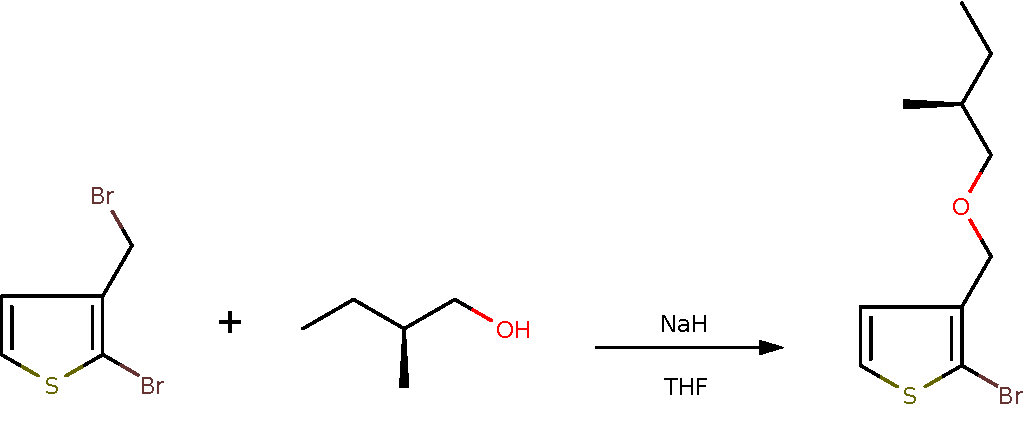
\includegraphics[scale=0.5]
{syn1-eterificazione.pdf}
\end{figure}

2-methyl-1-butanol (\SI{0.26}{\mL}, \SI{210}{\mg}, \SI{2.4}{\mmol}) distilled on calcium oxide was dissolved in dry tetrahydrofuran (\SI{6}{\mL}) in a Schlenk tube under nitrogen atmosphere. The reaction was cooled to \SI{0}{\celsius} and sodium hydride (\SI{55}{\mg}, \SI{2.3}{\mmol}) was added in portions. After stirring at room temperature for \SI{30}{\minute} the reaction was cooled to \SI{0}{\celsius} and 2-bromo-3-(bromo\-methyl)\-thio\-phene (\SI{0.26}{\mL}, \SI{510}{\mg}, \SI{2}{\mmol}) was added. The reaction mixture was stirred for \SI{40}{\minute} at \SI{0}{\celsius}, then at room temperature overnight. 
The reaction was quenched by adding water and extracted with dichloromethane (3 $\times$ \SI{8}{\mL}). Organic fractions were washed with water and purified through flash column chromatography (silica gel, heptane:\-di\-chloro\-methane 4:1, dry deposition) obtaining 2-bromo-3-[(2-methyl\-butyl\-oxy)\-methyl{]}\-thio\-phene \cmpd+{ig2-9} as a colorless oil (\SI{348.7}{\mg}, yield 66~\%, \gls{GCMS} pure). 

\gls{GCMS} (EI): 262, 264 (\ch{M+}), 174.9, 176.9 (\ch{M+ $-$ OC5H11}), 113.0 (\ch{M+ $-$ C5H11 $-$ Br + H}), 97.0 (\ch{M+ $-$ OC5H11 $-$ Br + H}).

\subsection[2-bromo-3-[((S)-2-methyl\-butyl\-oxy)\-methyl{]}\-thio\-phene (\cmpd+{ig2-1})]{2-bromo-3-[((S)-2-methyl\-butyl\-oxy)\-methyl{]}\-thio\-phene (\cmpd+{ig2-1}) \\ Etherification of 2-bromo-3-(bromo\-methyl)\-thio\-phene with (S)-2-methyl-1-butanol}%SDIG2-1
\label{sec:ig2-1}
The synthetic procedure for 2-bromo-3-[(2-methyl\-butyl\-oxy)\-methyl{]}\-thio\-phene \cmpd+{ig2-9} was followed using 2-bromo-3-(bromo\-methyl)\-thio\-phene (\SI{0.67}{\mL}, \SI{1.3}{\g}, \SI{5.2}{\mmol}), (S)-2-methyl-1-butanol (without further purification, \SI{0.704}{\mL}, \SI{0.577}{\g}, \SI{6.54}{\mmol}), sodium hydride (\SI{0.140}{\g}, \SI{5.82}{\mmol}) and tetrahydrofuran (\SI{15}{\mL}). The crude product was extracted with dichloromethane and water, then was purified by silica gel column chromatography (hexane:\-chloro\-form 4:1) affording 2-bromo-3-[((S)-2-methyl\-butyl\-oxy)\-methyl{]}\-thio\-phene \cmpd+{ig2-1} as a colorless oil (\SI{0.959}{\g}, yield 71~\%, \gls{GCMS} pure).

\gls{GCMS} (EI): 262, 264 (\ch{M+}), 174.9, 176.9 (\ch{M+ $-$ OC5H11}), 113.0 (\ch{M+ $-$ C5H11 $-$ Br + H}), 97.0 (\ch{M+ $-$ OC5H11 $-$ Br + H}).

\subsection[2-bromo-5-iodo-3-[(2-methyl\-butyl\-oxy)\-methyl{]}\-thio\-phene (\cmpd+{ig2-10})]{2-bromo-5-iodo-3-[(2-methyl\-butyl\-oxy)\-methyl{]}\-thio\-phene (\cmpd+{ig2-10}) \\ Iodination of 2-bromo-3-[(2-methyl\-butyl\-oxy)\-methyl{]}\-thio\-phene}
\label{sec:ig2-10}

\begin{figure}[H]%syn2-iodurazione
\centering
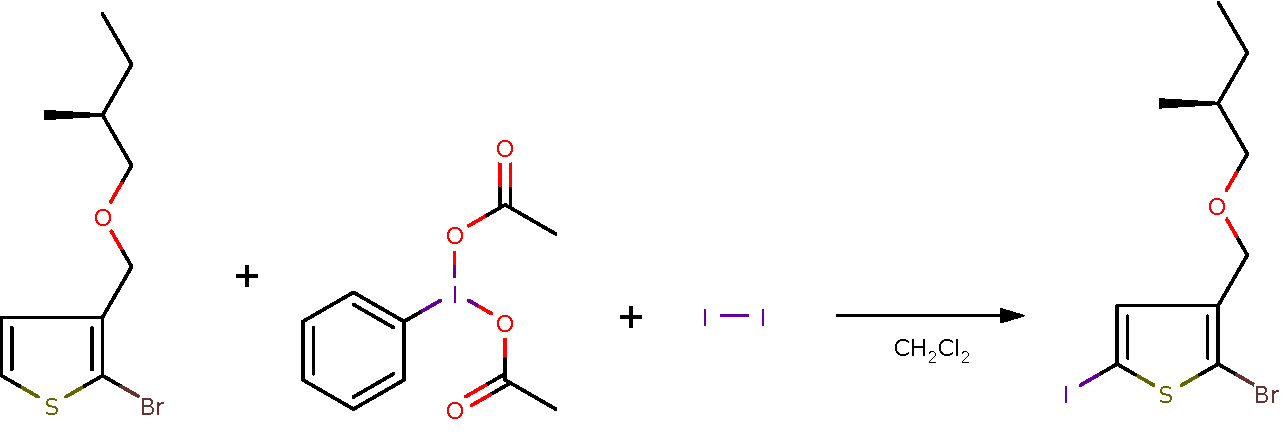
\includegraphics[scale=0.5]
{syn2-iodurazione.pdf}
\end{figure}

In a Schlenk tube 2-bromo-3-[(2-methyl\-butyl\-oxy)\-methyl{]}\-thio\-phene \cmpd+{ig2-1} (\SI{349}{\mg}, \SI{1.32}{\mmol}) was dried with mechanical pump and kept under nitrogen atmosphere. Dichloromethane (\SI{3}{\mL}, degassed by bubbling nitrogen) was added and the flask was cooled to \SI{0}{\celsius}. Iodine (\SI{219}{\mg}, \SI{0.864}{\mmol}) and iodo\-benzene di\-acetate (\ch{PhI(OAc)2}, \SI{255}{\mg}, \SI{0.79}{\mmol}) were added and the reaction was stirred at \SI{0}{\celsius} for \SI{4}{\hour}. 
The reaction was quenched with saturated aqueous sodium thio\-sulfate (\SI{5}{\mL}) keeping the temperature at \SI{0}{\celsius}. Then was extracted with dichloromethane (4 $\times$ \SI{10}{\mL}) and the organic fractions were washed with water. The product was purified by a flash chromatography on silica gel (hexane:\-chloro\-form 9:1, dry deposition). 
The selected fractions were concentrated and purified through a second flash column chromatography (hexane:\-ethyl\-acetate 69:1, dry deposition) to obtain a pale yellow oil (\SI{484.6}{\mg}). \gls{GCMS} analysis on the obtained oil showed the presence of the desired product 2-bromo-5-iodo-3-[(2-methyl\-butyl\-oxy)\-methyl{]}\-thio\-phene \cmpd+{ig2-10} (94~\% in oil, 93~\% overall yield) together with an impurity of 2-bromo-4,5-diiodo-3-[(2-methyl\-butyl\-oxy)\-methyl{]}\-thio\-phene (6~\% in oil).

{\HNMR} (\SI{600}{\MHz}, \gls{TCE}-d$_2$) $\delta$ (ppm) 7.13 (s, 1H, arom.\ H), 4.31 (s, 2H, \ch{CCH2O}), 3.26 (dd, $J =$ \SI{9.1}{\Hz} (geminal), \SI{6.3}{\Hz}, 1H, \ch{OC\underline{H}2CH}), 3.17 (dd, $J =$ \SI{8.9}{\Hz} (geminal), \SI{7.0}{\Hz}, 1H, \ch{OC\underline{H}2CH}), 1.61 (m, 1H, \ch{OCH2C\underline{H}}), 1.40 (m, 1H, \ch{OCH2CHC\underline{H}2}), 1.09 (m, 1H, \ch{OCH2CHC\underline{H}2}), 0.85 (d, $J =$ \SI{6.6}{\Hz}, 3H, \ch{CHC\underline{H}3}), 0.84 (t, $J =$ \SI{7.4}{\Hz}, 3H, \ch{CH2C\underline{H}3}).
{\CNMR} (\SI{150}{\MHz}, \gls{TCE}-d$_2$) $\delta$ (ppm) 141.01 (arom.\ \ch{\underline{C}CH2}), 137.81 (arom.\ \ch{CH}), 113.05 (\ch{CBr}), 75.80 (\ch{O\underline{C}H2CH}), 71.86 (\ch{CI}), 66.36 (\ch{C\underline{C}H2O}), 34.69 (\ch{OCH2\underline{C}H}), 26.08 (\ch{OCH2CH\underline{C}H2}), 16.52 (\ch{CH\underline{C}H3}), 11.30 (\ch{CH2\underline{C}H3}).
\gls{GCMS} (EI): 387.9, 389.9 (\ch{M+}), 300.8, 302.8 (\ch{M+ $-$ OC5H11}), 222.9 (\ch{M+ $-$ C5H11 $-$ Br + H}), 174.9, 176.9 (\ch{M+ $-$ C5H11 $-$ I + H}).
\gls{FTIR} (film on \ch{KBr}) $\nu$ (\SI{}{\per\cm}) 3093 (weak, arom.\ CH stretching), 2959 (strong, \ch{CH3} degen.\ stretching), 2928 (strong, \ch{CH2} antisymm.\ stretching), 2873 (strong, \ch{CH3} symm.\ stretching), 2858 (strong, \ch{CH2} symm.\ stretching), 1461 (medium, \ch{C=C} thiophene symm.\ stretching, \ch{CH3} degen.\ deform.), 1413 (medium), 1178 (medium), 1098 (strong, \ch{CO} antisymm.\ stretching), 994 (medium, ring breathing), 833 (medium, arom.\ H out-of-plane bending), 471.

\subsection[2-bromo-5-iodo-3-[((S)-2-methyl\-butyl\-oxy)\-methyl{]}\-thio\-phene (\cmpd+{ig2-2})]{2-bromo-5-iodo-3-[((S)-2-methyl\-butyl\-oxy)\-methyl{]}\-thio\-phene (\cmpd+{ig2-2}) \\ Iodination of 2-bromo-3-[((S)-2-methyl\-butyl\-oxy)\-methyl{]}\-thio\-phene}
\label{sec:ig2-2}
The synthetic procedure for 2-bromo-5-iodo-3-[(2-methyl\-butyl\-oxy)\-methyl{]}\-thio\-phene \cmpd+{ig2-10} was followed using 2-bromo-3-[((S)-2-methyl\-butyl\-oxy)\-methyl{]}\-thio\-phene \cmpd+{ig2-1} (\SI{0.959}{\g}, \SI{3.64}{\mmol}), iodine (\ch{I2}, \SI{0.601}{\g}, \SI{2.37}{\mmol}), iodo\-benzene di\-acetate (\ch{PhI(OAc)2}, \SI{0.700}{\g}, \SI{2.17}{\mmol}) and dichloromethane (\SI{8}{\mL}). 
The crude product was extracted with dichloromethane and water, then was purified by two following silica gel column chromatographies (hexane:\-chloro\-form 9:1, then hexane:\-ethyl acetate 69:1) affording 2-bromo-5-iodo-3-[((S)-2-methyl\-butyl\-oxy)\-methyl{]}\-thio\-phene \cmpd+{ig2-2} as a pale yellow oil (\SI{1.343}{\g}, yield 95~\%, \gls{GCMS} pure, {\HNMR} pure).

{\HNMR} (\SI{600}{\MHz}, \gls{TCE}-d$_2$) $\delta$ (ppm) 7.12 (s, 1H, arom.\ H), 4.31 (s, 2H, \ch{CCH2O}), 3.25 (dd, $J =$ \SI{9.1}{\Hz} (geminal), \SI{6.2}{\Hz}, 1H, \ch{OC\underline{H}2CH}), 3.17 (dd, $J =$ \SI{9.1}{\Hz} (geminal), \SI{6.9}{\Hz}, 1H, \ch{OC\underline{H}2CH}), 1.61 (m, 1H, \ch{OCH2C\underline{H}}), 1.39 (m, 1H, \ch{OCH2CHC\underline{H}2}), 1.08 (m, 1H, \ch{OCH2CHC\underline{H}2}), 0.85 (d, $J =$ \SI{6.7}{\Hz}, 3H, \ch{CHC\underline{H}3}), 0.84 (t, $J =$ \SI{7.4}{\Hz}, 3H, \ch{CH2C\underline{H}3}).
{\HNMR} (\SI{600}{\MHz}, \ch{CDCl3}) $\delta$ (ppm) 7.15 (s, 1H, arom.\ H), 4.37 (s, 2H, \ch{CCH2O}), 3.31 (dd, $J =$ \SI{9.0}{\Hz} (geminal), \SI{6.2}{\Hz}, 1H, \ch{OC\underline{H}2CH}), 3.22 (dd, $J =$ \SI{9.0}{\Hz} (geminal), \SI{6.7}{\Hz}, 1H, \ch{OC\underline{H}2CH}), 1.66 (m, 1H, \ch{OCH2C\underline{H}}), 1.45 (m, 1H, \ch{OCH2CHC\underline{H}2}), 1.14 (m, 1H, \ch{OCH2CHC\underline{H}2}), 0.91 (d, $J =$ \SI{6.7}{\Hz}, 3H, \ch{CHC\underline{H}3}), 0.89 (t, $J =$ \SI{7.5}{\Hz}, 3H, \ch{CH2C\underline{H}3}). 
{\CNMR} (\SI{150}{\MHz}, \ch{CDCl3}) $\delta$ (ppm) 141.10 (arom.\ \ch{\underline{C}CH2}), 137.97 (arom.\ \ch{CH}), 113.41 (\ch{CBr}), 76.05 (\ch{O\underline{C}H2CH}), 71.97 (\ch{CI}), 66.68 (\ch{C\underline{C}H2O}), 35.09 (\ch{OCH2\underline{C}H}), 26.34 (\ch{OCH2CH\underline{C}H2}), 16.73 (\ch{CH\underline{C}H3}), 11.43 (\ch{CH2\underline{C}H3}).
\gls{GCMS} (EI): 387.9, 389.9 (\ch{M+}), 300.8, 302.8 (\ch{M+ $-$ OC5H11}), 222.9 (\ch{M+ $-$ C5H11 $-$ Br + H}), 174.9, 176.9 (\ch{M+ $-$ C5H11 $-$ I + H}).

\end{section}
\begin{section}{Polymerization}

\subsection[Poly\{3-[((S)-2-methyl\-butyl\-oxy)\-methyl{]}\-thio\-phene\} (\cmpd+{ig2-4})]{Poly\{3-[((S)-2-methyl\-butyl\-oxy)\-methyl{]}\-thio\-phene\} (\cmpd+{ig2-4}) \\ Polymerization of 2-bromo-5-iodo-3-[((S)-2-methyl\-butyl\-oxy)\-methyl{]}\-thio\-phene}
\label{sec:ig2-4}

\begin{figure}[H]%syn3-attivazione-nolicl
\centering
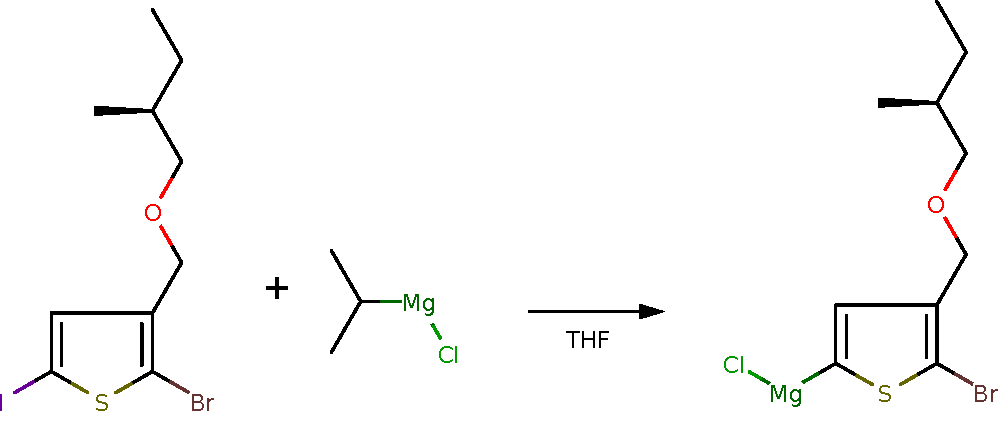
\includegraphics[scale=0.5]
{syn3-attivazione-nolicl.pdf}
\smallskip

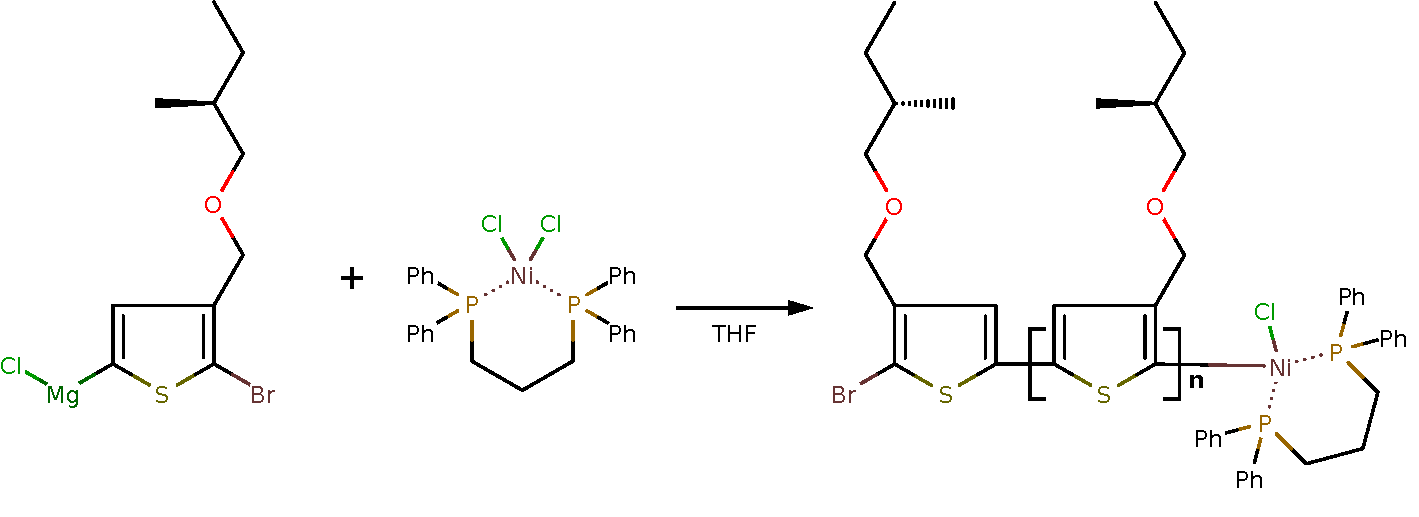
\includegraphics[scale=0.5]
{syn4-polimerizzazione-nolicl.pdf}

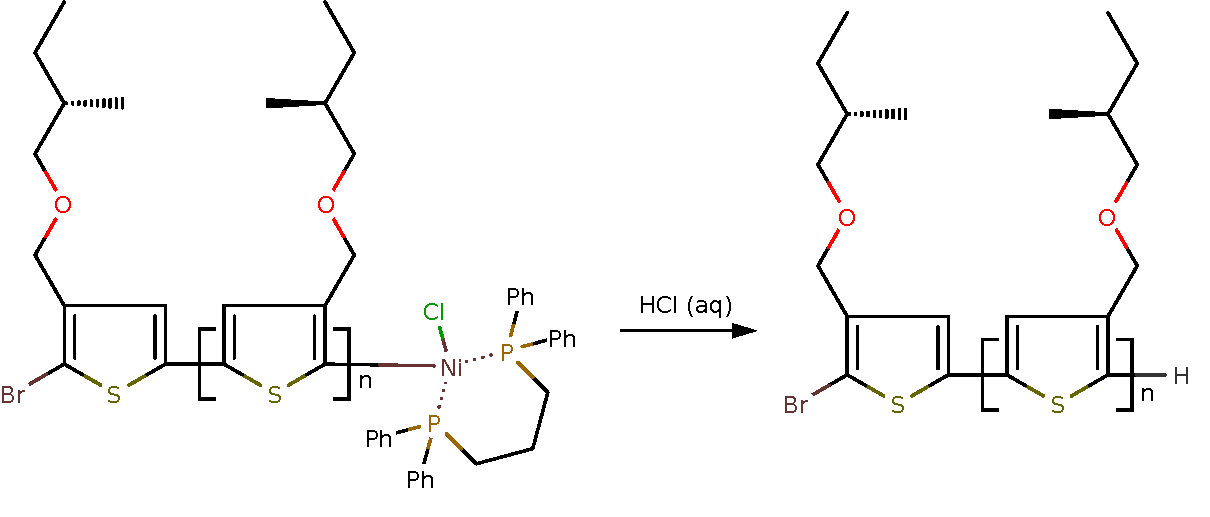
\includegraphics[scale=0.5]
{syn5-quenching.pdf}
\end{figure}
2-bromo-5-iodo-3-[((S)-2-methyl\-butyl\-oxy)\-methyl{]}\-thio\-phene \cmpd+{ig2-2} (\SI{266}{\mg}, \SI{0.684}{\mmol}) was placed in a Schlenk tube under nitrogen atmosphere. Then dry tetrahydrofuran (\SI{4}{\mL}) was added, the reaction mixture was cooled to \SI{0}{\celsius} and isopropyl-magnesium chloride (\SI{2.0}{\Molar} solution in tetrahydrofuran, \SI{0.34}{\mL}, \SI{0.68}{\mmol}) was added dropwise. The mixture was stirred at \SI{0}{\celsius} for \SI{1}{\hour}, then a suspension of \acrlong{nidppp} (\acrshort{nidppp}, \SI{6.0}{\mg}, \SI{0.011}{\mmol}%
) in dry tetrahydrofuran (\SI{3}{\mL}) was added in one portion, then was stirred at room temperature for \SI{24}{\hour}.
The reaction was quenched by adding aqueous hydrochloric acid (\SI{5}{\Molar}, \SI{11}{\mL}), then was extracted with chloroform (\SI{200}{\mL}). The organic fraction was reduced to few milliliters, precipitated from methanol (\SI{0.5}{\L}) and filtered (\gls{PTFE} membrane, \SI{0.45}{\um}).
The solid was washed with hot methanol (\SI{50}{\celsius}), dried under reduced pressure and recovered mechanically from the filter, redissolved in chloroform, re\-precipitated in methanol and filtered again to obtain poly\{3-[((S)-2-methyl\-butyl\-oxy)\-methyl{]}\-thio\-phene\} \cmpd+{ig2-4} as a dark red solid (\SI{35}{\mg}, yield 22~\%). 

{\HNMR} (\SI{600}{\MHz}, \gls{TCE}-d$_2$) $\delta$ (ppm) 7.22 (s, 1H, arom.\ H), 4.54 (s, 2H, \ch{CCH2O}), 3.40 (m, 1H, \ch{OC\underline{H}2CH}), 3.31 (m, 1H, \ch{OC\underline{H}2CH}), 1.69 (m, 1H, \ch{OCH2C\underline{H}}), 1.47 (m, 1H, \ch{OCH2CHC\underline{H}2}), 1.15 (m, 1H, \ch{OCH2CHC\underline{H}2}), 0.94 -- 0.86 (m, 6H, \ch{CHC\underline{H}3 + CH2C\underline{H}3}).
{\HNMR} (\SI{600}{\MHz}, \ch{CDCl3}) $\delta$ (ppm) 7.25 (s, 1H, arom.\ H), 4.58 (s, 2H, \ch{CCH2O}), 3.45 -- 3.40 (m, 1H, \ch{OC\underline{H}2CH}), 3.36 -- 3.31 (m, 1H, \ch{OC\underline{H}2CH}), 1.85 -- 1.69 (m, 1H, \ch{OCH2C\underline{H}}), 1.57 -- 1.49 (m, 1H, \ch{OCH2CHC\underline{H}2}), 1.24 -- 1.15 (m, 1H, \ch{OCH2CHC\underline{H}2}), 0.99 -- 0.91 (m, 6H, \ch{CHC\underline{H}3 + CH2C\underline{H}3}).
{\CNMR} (\SI{150}{\MHz}, \gls{TCE}-d$_2$) $\delta$ (ppm) 136.54 (arom.\ \ch{\underline{C}CH2}), 133.68 (arom.\ \ch{S\underline{C}CCH2}), 132.91 (arom.\ \ch{S\underline{C}CH}), 129.28 (arom.\ \ch{CH}), 75.88 (\ch{O\underline{C}H2CH}), 66.71 (\ch{C\underline{C}H2O}), 34.86 (\ch{OCH2\underline{C}H}), 26.25 (\ch{OCH2CH\underline{C}H2}), 16.73 (\ch{CH\underline{C}H3}), 11.38 (\ch{CH2\underline{C}H3}).
{\CNMR} (\SI{100}{\MHz}, \ch{CDCl3}) $\delta$ (ppm) 136.61 (arom.\ \ch{\underline{C}CH2}), 134.25 (arom.\ \ch{S\underline{C}CCH2}), 133.36 (arom.\ \ch{S\underline{C}CH}), 129.52 (arom.\ \ch{CH}), 76.13 (\ch{O\underline{C}H2CH}), 67.02 (\ch{C\underline{C}H2O}), 35.23 (\ch{OCH2\underline{C}H}), 26.50 (\ch{OCH2CH\underline{C}H2}), 16.94 (\ch{CH\underline{C}H3}), 11.52 (\ch{CH2\underline{C}H3}).
$^1$H-COSY, $^1$H-TOCSY, $^1$H,$^{13}$C-HSQC and $^1$H,$^{13}$C-HMBC characterizations results are reported in table~\ref{tab:ig2-4-nmr2d}.
\gls{FTIR} (film on \ch{KBr}) $\nu$ (\SI{}{\per\cm}) 3064 (weak, arom.\ CH stretching), 2961 (strong, \ch{CH3} degen.\ stretching), 2930 (strong, \ch{CH2} antisymm.\ stretching), 2874 (strong, \ch{CH3} symm.\ stretching), 2858 (strong, \ch{CH2} symm.\ stretching), 2805 (medium), 2729 (weak), 1517 (medium), 1461 (medium, \ch{C=C} thiophene symm.\ stretching, \ch{CH3} degen.\ deform.), 1378 (medium, \ch{CH3} symm.\ deform.), 1180 (medium), 1091 (strong, \ch{CO} antisymm.\ stretching), 838 (medium, arom.\ H out-of-plane bending).

\vfill

\subsection[Poly\{3-[(2-methyl\-butyl\-oxy)\-methyl{]}\-thio\-phene\} (\cmpd+{ig2-15})]{Poly\{3-[(2-methyl\-butyl\-oxy)\-methyl{]}\-thio\-phene\} (\cmpd+{ig2-15}) \\ Polymerization of 2-bromo-5-iodo-3-[(2-methyl\-butyl\-oxy)\-methyl{]}\-thio\-phene in presence of \ch{LiCl}}
\label{sec:ig2-15}

\begin{figure}[H]%syn3-attivazione-licl
\centering
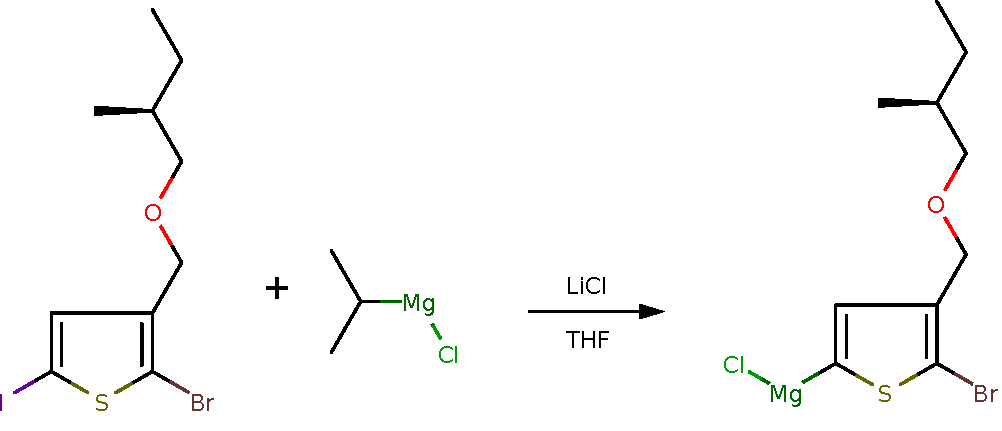
\includegraphics[scale=0.5]
{syn3-attivazione-licl.pdf}

\smallskip
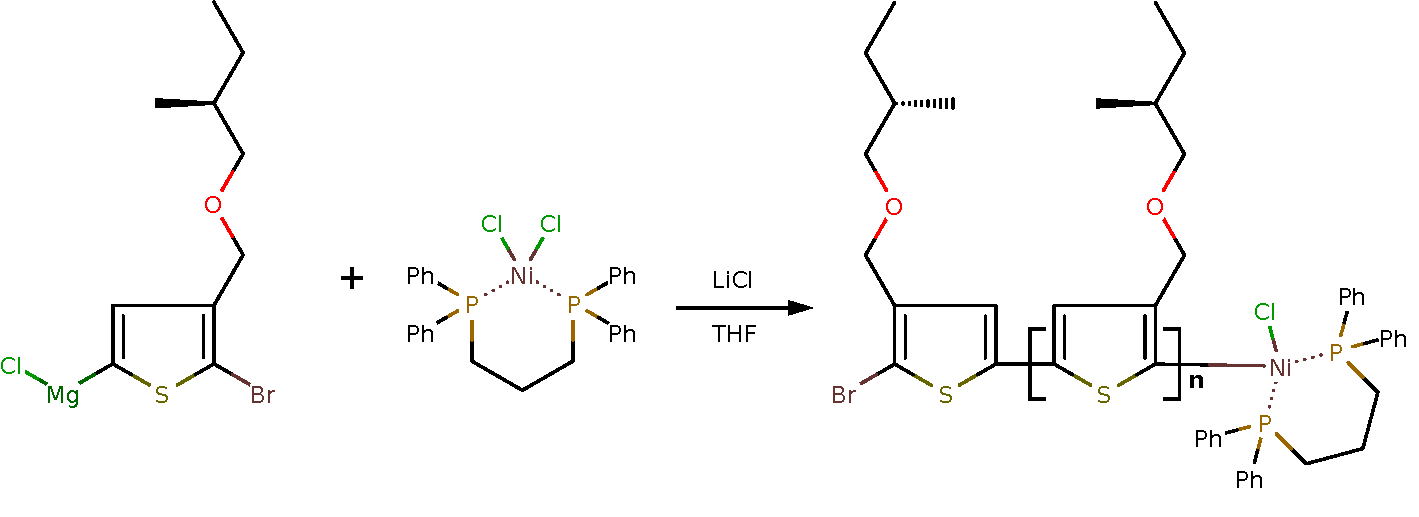
\includegraphics[scale=0.5]
{syn4-polimerizzazione-licl.pdf}

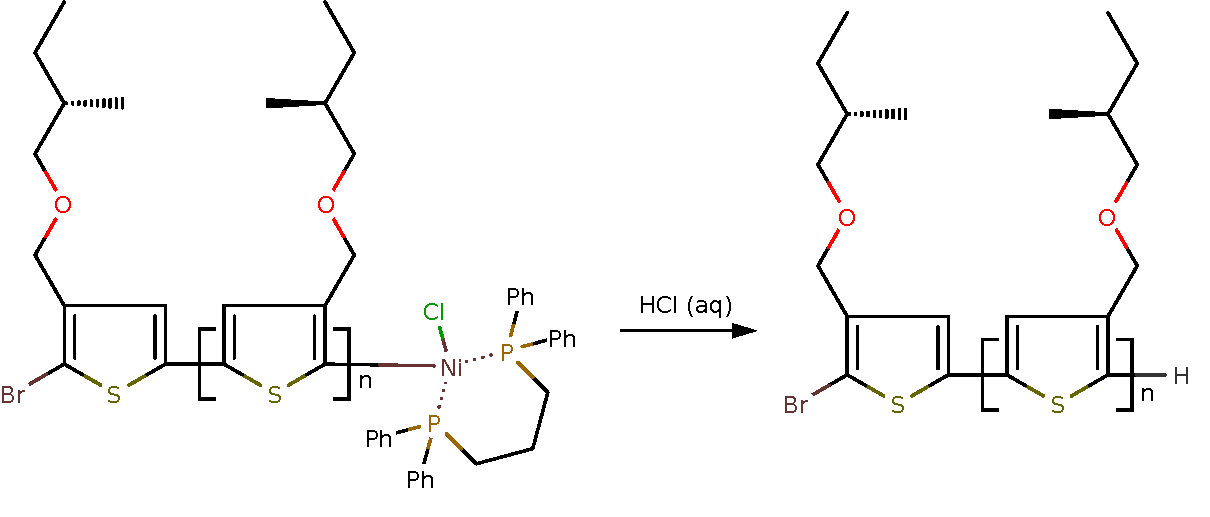
\includegraphics[scale=0.5]
{syn5-quenching.pdf}
\end{figure}
A Schlenk tube equipped with a septum and stirring bar was charged with lithium chloride (\SI{85}{\mg}, \SI{2}{\mmol}, hygroscopic) and was heated by a heat-gun under reduced pressure. After the tube was cooled to room temperature under a nitrogen atmosphere, 2-bromo-5-iodo-3-[(2-methyl\-butyl\-oxy)\-methyl{]}\-thio\-phene \cmpd+{ig2-10} (\SI{152}{\mg}, \SI{0.391}{\mmol}, optical purity 59~\%) was added and dried under reduced pressure (mechanical pump). 
Then dry tetrahydrofuran (\SI{6}{\mL}) was added, the reaction mixture was cooled to \SI{0}{\celsius} and iso\-propyl\-magnesium chloride (\SI{2.0}{\Molar} solution in tetrahydrofuran, \SI{0.20}{\mL}, \SI{0.40}{\mmol}) was added dropwise (\SI{2}{\minute}) while stirring. 
The mixture was stirred at \SI{0}{\celsius} for \SI{50}{\minute}, then a suspension of \acrlong{nidppp} (\acrshort{nidppp}, \SI{4.84}{\mg}, \SI{8.93}{\umol}) in dry tetrahydrofuran (\SI{1.29}{\mL}) was added in one portion. 
The reaction was stirred at \SI{0}{\celsius} for \SI{2}{\minute} and at room temperature overnight. The polymerization was quenched by the rapid addition of aqueous hydrochloric acid (\SI{5}{\Molar}, \SI{4}{\mL}) and extracted with chloroform (4 $\times$ \SI{2}{\mL}). The collected organic fractions were washed with water (2 $\times$ \SI{7}{\mL}) and the solvent removed under reduced pressure. 
The resulting red solid was fractionated by Soxhlet extraction using methanol (extracted \SI{26}{\mg}), heptane (extracted \SI{3}{\mg}) and acetone (extracted \SI{3}{\mg}), and finally recovered using chloroform. The solvent was removed under reduced pressure to give poly\{3-[(2-methyl\-butyl\-oxy)\-methyl{]}\-thio\-phene\} \cmpd+{ig2-15} as a dark red solid (\SI{43.3}{\mg}, yield 61~\%).

{\HNMR} (\SI{600}{\MHz}, \gls{TCE}-d$_2$) $\delta$ (ppm) 7.21 (s, 1H, arom.\ H), 4.55 (s, 2H, \ch{CCH2O}), 3.40 (dd, $J =$ \SI{8.8}{\Hz} (geminal), \SI{6.2}{\Hz}, 1H, \ch{OC\underline{H}2CH}), 3.31 (dd, $J =$ \SI{9.1}{\Hz} (geminal), \SI{6.8}{\Hz}, 1H, \ch{OC\underline{H}2CH}), 1.74 -- 1.63 (m, 1H, \ch{OCH2C\underline{H}}), 1.53 -- 1.41 (m, 1H, \ch{OCH2CHC\underline{H}2}), 1.18 -- 1.08 (m, 1H, \ch{OCH2CHC\underline{H}2}), 0.92 (d, $J =$ \SI{6.7}{\Hz}, 3H, \ch{CHC\underline{H}3}), 0.88 (t, $J =$ \SI{7.4}{\Hz}, 3H, \ch{CH2C\underline{H}3}).
{\CNMR} (\SI{150}{\MHz}, \gls{TCE}-d$_2$) $\delta$ (ppm) 136.55 (arom.\ \ch{\underline{C}CH2}), 133.68 (arom.\ \ch{S\underline{C}CCH2}), 132.90 (arom.\ \ch{S\underline{C}CH}), 129.28 (arom.\ \ch{CH}), 75.88 (\ch{O\underline{C}H2CH}), 66.71 (\ch{C\underline{C}H2O}), end of spectral window.
\gls{FTIR} (film on \ch{KBr}) $\nu$ (\SI{}{\per\cm}) 3061, 2961, 2927, 2874, 2858, 2805, 1462, 1378, 1261, 1091, 1019, 841, 801.

\subsection[Poly\{3-[((S)-2-methyl\-butyl\-oxy)\-methyl{]}\-thio\-phene\} (\cmpd+{ig2-8})]{Poly\{3-[((S)-2-methyl\-butyl\-oxy)\-methyl{]}\-thio\-phene\} (\cmpd+{ig2-8}) \\ Polymerization of 2-bromo-5-iodo-3-[((S)-2-methyl\-butyl\-oxy)\-methyl{]}\-thio\-phene in presence of \ch{LiCl}}
\label{sec:ig2-8}
The synthetic procedure for poly\{3-[(2-methyl\-butyl\-oxy)\-methyl{]}\-thio\-phene\} \cmpd+{ig2-15} was followed using 2-bromo-5-iodo-3-[((S)-2-methyl\-butyl\-oxy)\-methyl{]}\-thio\-phene \cmpd+{ig2-2} (\SI{312}{\mg}, \SI{0.802}{\mmol}%
), lithium chloride (\SI{176}{\mg}, \SI{4.15}{\mmol}), iso\-propyl\-magnesium chloride (\SI{0.400}{\mL}, \SI{0.800}{\mmol}%
), \acrlong{nidppp} (\acrshort{nidppp}, \SI{9.8}{\mg}, \SI{0.018}{\mmol}%
), and tetrahydrofuran (\SI{20}{\mL}). 
The crude product was extracted with chloroform and water, the collected organic fractions were dried under reduced pressure and fractionated by Soxhlet extraction using methanol (extracted \SI{52.5}{\mg}), hexane (extracted \SI{9}{\mg}) and acetone (extracted \SI{4}{\mg}), and finally recovered using chloroform. After solvent evaporation poly\{3-[((S)-2-methyl\-butyl\-oxy)\-methyl{]}\-thio\-phene\} was obtained as a dark red solid \cmpd+{ig2-8} (\SI{113.6}{\mg}, yield 78~\%%
).

{\HNMR} (\SI{600}{\MHz}, \gls{TCE}-d$_2$) $\delta$ (ppm) 7.21 (s, 1H, arom.\ H), 4.54 (s, 2H, \ch{CCH2O}), 3.40 (dd, $J =$ \SI{9.0}{\Hz} (geminal), \SI{6.1}{\Hz}, 1H, \ch{OC\underline{H}2CH}), 3.31 (dd, $J =$ \SI{8.8}{\Hz} (geminal), \SI{7.0}{\Hz}, 1H, \ch{OC\underline{H}2CH}), 1.77 -- 1.59 (m, 1H, \ch{OCH2C\underline{H}}), 1.52 -- 1.36 (m, 1H, \ch{OCH2CHC\underline{H}2}), 1.19 -- 1.05 (m, 1H, \ch{OCH2CHC\underline{H}2}), 0.92 (d, $J =$ \SI{6.5}{\Hz}, 3H, \ch{CHC\underline{H}3}), 0.88 (t, $J =$ \SI{7.3}{\Hz}, 3H, \ch{CH2C\underline{H}3}).
{\CNMR} (\SI{150}{\MHz}, \gls{TCE}-d$_2$) $\delta$ (ppm) 136.55 (arom.\ \ch{\underline{C}CH2}), 133.68 (arom.\ \ch{S\underline{C}CCH2}), 132.90 (arom.\ \ch{S\underline{C}CH}), 129.28 (arom.\ \ch{CH}), 75.88 (\ch{O\underline{C}H2CH}), 66.71 (\ch{C\underline{C}H2O}), 34.86 (\ch{OCH2\underline{C}H}), 26.25 (\ch{OCH2CH\underline{C}H2}), 16.73 (\ch{CH\underline{C}H3}), 11.38 (\ch{CH2\underline{C}H3}).
\gls{FTIR} (film on \ch{KBr}) $\nu$ (\SI{}{\per\cm}) 3062, 2961, 2928, 2874, 2858, 2805, 1462, 1378, 1091, 841. 

\end{section}
\begin{section}{Synthesis of Mediator for Radical Polimerization}

\subsection[1-(4-Bromo\-phenyl)\-ethanol (\cmpd+{ig2-16})]{1-(4-Bromo\-phenyl)\-ethanol (\cmpd+{ig2-16}) \\ Reduction of 4-bromo\-aceto\-phenone}%SDIG2-16

\begin{figure}[H]%syn6-riduzione
\centering
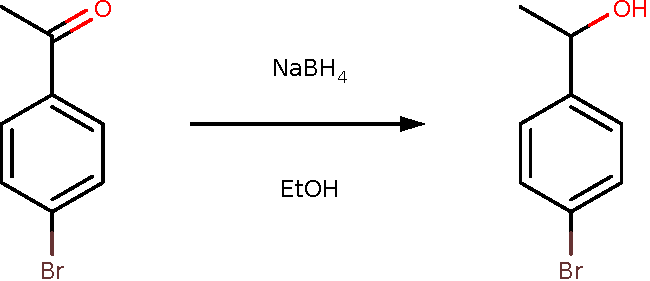
\includegraphics[scale=0.5]
{syn6-riduzione.pdf}
\end{figure}

Sodium boro\-hydride (\ch{NaBH4}, \SI{57}{\mg}, \SI{1.5}{\mmol}) was added to a stirred solution of 4-bromo\-aceto\-phenone (\SI{203}{\mg}, \SI{1}{\mmol}) in ethanol (reagent grade, \SI{10}{\mL}). After stirring for \SI{4}{\hour} the reaction mixture was concentrated in mild vacuum and the residue dissolved in dichloromethane (\SI{30}{\mL}). The organic layer was subsequently washed with distilled water (3 $\times$ \SI{20}{\mL}), the organic extract was concentrated in mild vacuum to afford 1-(4-bromo\-phenyl)\-ethanol \cmpd+{ig2-16} (\SI{155}{\mg}, yield 76~\%, \gls{GCMS} pure). 

\gls{GCMS} (EI): 202.0, 204.0 (\ch{M+}), 184.9, 186.9 (\ch{M+ $-$ CH3}), 156.9, 158.9, 121.1 (\ch{M+ $-$ Br}), 103 (\ch{M+ $-$ Br $-$ H2O}).

\subsection[1-Bromo-4-(1-bromo\-ethyl)\-benzene (\cmpd+{ig2-17})]{1-Bromo-4-(1-bromo\-ethyl)\-benzene (\cmpd+{ig2-17}) \\ Bromination of 1-(4-bromo\-phenyl)\-ethanol}

\begin{figure}[H]%syn7-bromurazione
\centering
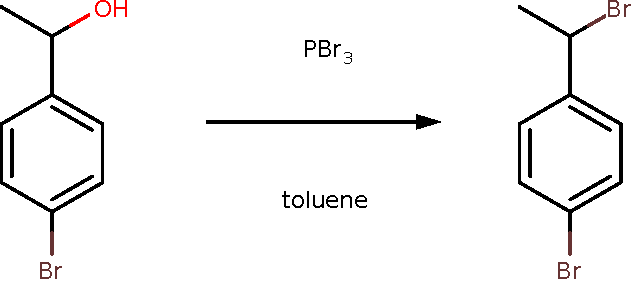
\includegraphics[scale=0.5]
{syn7-bromurazione.pdf}
\end{figure}

In a \SI{25}{\mL} Schlenk tube phosphorus tri\-bromide (\ch{PBr3}, \SI{60}{\uL}, \SI{0.64}{\mmol}) was dissolved in toluene dry (\SI{4}{\mL}, this solution showed some white precipitate at first, then turned to pale yellow). 
\SI{2}{\mL} of the previously prepared phosphorus tri\-bromide solution were added drop wise (\SI{10}{\minute}) to a solution of 1-(4-bromo\-phenyl)\-ethanol \cmpd+{ig2-16} (\SI{155}{\mg}, \SI{0.771}{\mmol} in a \SI{25}{\mL} Schlenk tube) in toluene dry (about \SI{2}{\mL}) at \SI{-5}{\celsius} (cooled using an immersion cooler in a external bath). The reaction was stirred for \SI{4}{\hour} keeping at \SI{-5}{\celsius}, then it was quenched with water.
The organic layer was separated and the aqueous layer was extracted with diethyl ether (2 $\times$ \SI{15}{\mL}). The organic layers were collected and washed with water (\SI{10}{\mL}), dried over anhydrous magnesium sulfate, filtered and concentrated under reduced pressure (\SI{40}{\celsius}, \SI{30}{\milli\bar}, then nitrogen flux) obtaining a pale pink oil (\SI{138}{\mg}). From \gls{GCMS} analysis the product results to be a mixture of 1-bromo-4-(1-bromo\-ethyl)\-benzene \cmpd+{ig2-17} (peak area 55~\%, \SI{76}{\mg}, \SI{0.29}{\mmol},
yield 37~\%) and 4-bromo\-styrene (peak area 45~\%, \SI{62}{\mg}, \SI{0.34}{\mmol}, 
yield 44~\%).

\gls{GCMS} (EI): 263.9 (\ch{M+}), 248.8 (\ch{M+ $-$ CH3}), 183.0, 185.0 (\ch{M+ $-$ Br}), 169, 171 (\ch{M+ $-$ Br $-$ CH2}), 155.9, 157.9 (\ch{M+ $-$ Br $-$ CCH3}), 104.1 (\ch{M+ $-$ Br $-$ Br}).

\subsection[\textit{N-Tert}-butyl-\textit{N}-(2-methyl-1-phenyl\-propyl)-\textit{O}-(1-phenyl\-ethyl)\-hydroxyl\-amine (\cmpd+{ig2-21})]{\textit{N-Tert}-butyl-\textit{N}-(2-methyl-1-phenyl\-propyl)-\textit{O}-(1-phenyl\-ethyl)\-hydroxyl\-amine (\cmpd+{ig2-21}) \\ Condensation of 1-bromo-4-(1-bromo\-ethyl)\-benzene with 2,2,5-tri\-methyl-4-phenyl-3-aza\-hexane-3-nitroxide}

\begin{figure}[H]%syn8-tipno-br
\centering
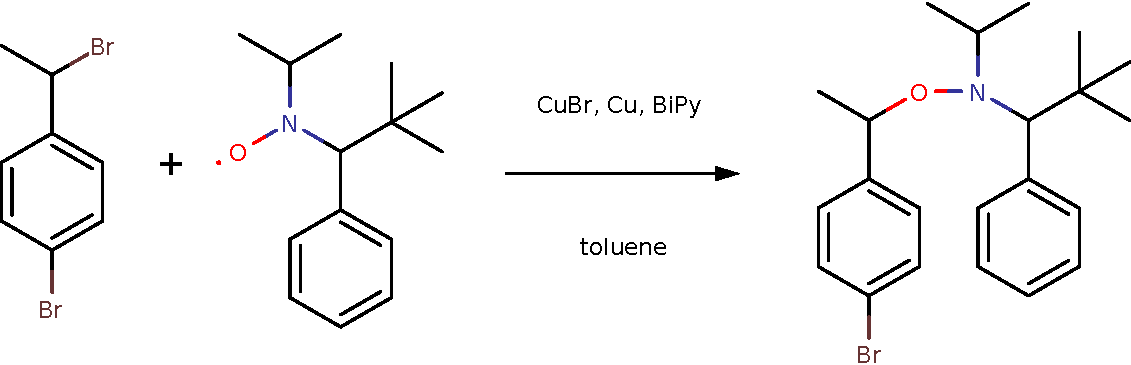
\includegraphics[scale=0.5]
{syn8-tipno-br.pdf}
\end{figure}

In a \SI{10}{\mL} Schlenk tube copper(I) bromide (\SI{17}{\mg}, \SI{0.12}{\mmol}), copper powder (\SI{547}{\mg}, \SI{8.61}{\mmol}) and 2,2'-bi\-pyridine (\SI{84}{\mg}, \SI{0.54}{\mmol}) were degassed under reduced pressure and dry toluene was added (\SI{8}{\mL}) obtaining a suspension.
To a solution of the crude 1-bromo-4-(1-bromo\-ethyl)\-benzene \cmpd+{ig2-17} (\SI{530}{\mg}, according \gls{GCMS} contains 55~\% 1-bromo-4-(1-bromo\-ethyl)\-benzene, \SI{1.10}{\mmol} and 45~\% of 4-bromo\-styrene, \SI{1.30}{\mmol}, in \SI{3}{\mL} toluene dry) toluene dry (\SI{10}{\mL}) and 2,2,5-tri\-methyl-4-phenyl-3-aza\-hexane-3-nitr\-oxide (\gls{TIPNO} radical, \SI{0.600}{\mL}, \SI{571}{\mg}, \SI{2.60}{\mmol}) were added. 
Then this mixture was degassed by bubbling nitrogen and \SI{1.88}{\mL} of the previously prepared suspension was added dropwise. After stirring the reaction mixture for \SI{24}{\hour} at \SI{75}{\celsius} (the suspension remained dark yellow rather turning to green as expected), the reaction was cooled down, adsorbed on basic allumina and filtered over basic alumina (column diameter \SI{2}{\cm}, height \SI{10}{\cm}), using hexane as the eluent to obtain \acrfull{BrPhEtTIPNO} \cmpd+{ig2-21} as a viscous colorless oil (\SI{333}{\mg}, from \gls{GCMS} and {\HNMR} analysis the product resulted to be a mixture with 10~\% of precursor \cmpd+{ig2-17} and 20~\% of di\-merized precursor isomers \ch{(BrC6H4C2H4)2}, so the yield in \cmpd+{ig2-21} was $\approx 50$~\%).

{\HNMR} (\SI{600}{\MHz}, \gls{TCE}-d$_2$) $\delta$ (ppm) 7.46 – 7.09 (m, 18H, arom.\ H), 4.83 (q, $J =$ \SI{6.6}{\Hz}, 1H, \ch{CHO}), 4.81 (q, $J =$ \SI{6.6}{\Hz}, 1H, \ch{CHO}), 3.35 (d, $J =$ \SI{10.6}{\Hz} (geminal), 1H, \ch{CHN}), 3.26 (d, $J =$ \SI{10.8}{\Hz} (geminal), 1H, \ch{CHN}), 2.24 (m, 1H, \ch{C\underline{H}(CH3)2}), 1.55 (d, $J =$ \SI{6.7}{\Hz}, 3H, \ch{CH(C\underline{H}3)2}), 1.47 (d, $J =$ \SI{6.6}{\Hz}, 3H, \ch{CH(C\underline{H}3)2}), 1.37 (m, 1H, \ch{C\underline{H}(CH3)2}), 1.24 (d, $J =$ \SI{6.3}{\Hz}, 3H, \ch{OCHC\underline{H}3}), 0.98 (s, 9H, \ch{C(C\underline{H}3)3}), 0.89 (d, $J =$ \SI{6.2}{\Hz}, 3H, \ch{OCHC\underline{H}3}), 0.72 (s, 9H, \ch{C(C\underline{H}3)3}), 0.48 (d, $J =$ \SI{6.6}{\Hz}, 3H, \ch{CH(C\underline{H}3)2}), 0.21 (d, $J =$ \SI{6.6}{\Hz}, 3H, \ch{CH(C\underline{H}3)2}).

\end{section}
\begin{section}[Second Block Polymerization]{Functionalization of Polythiophene as Macroinitiator and Second Block Polymerization}

\subsection{End-functionalization of Polythiophene with Aldehyde (\cmpd+{ig2-19})}

\begin{figure}[H]%syn9-suzuki
\centering
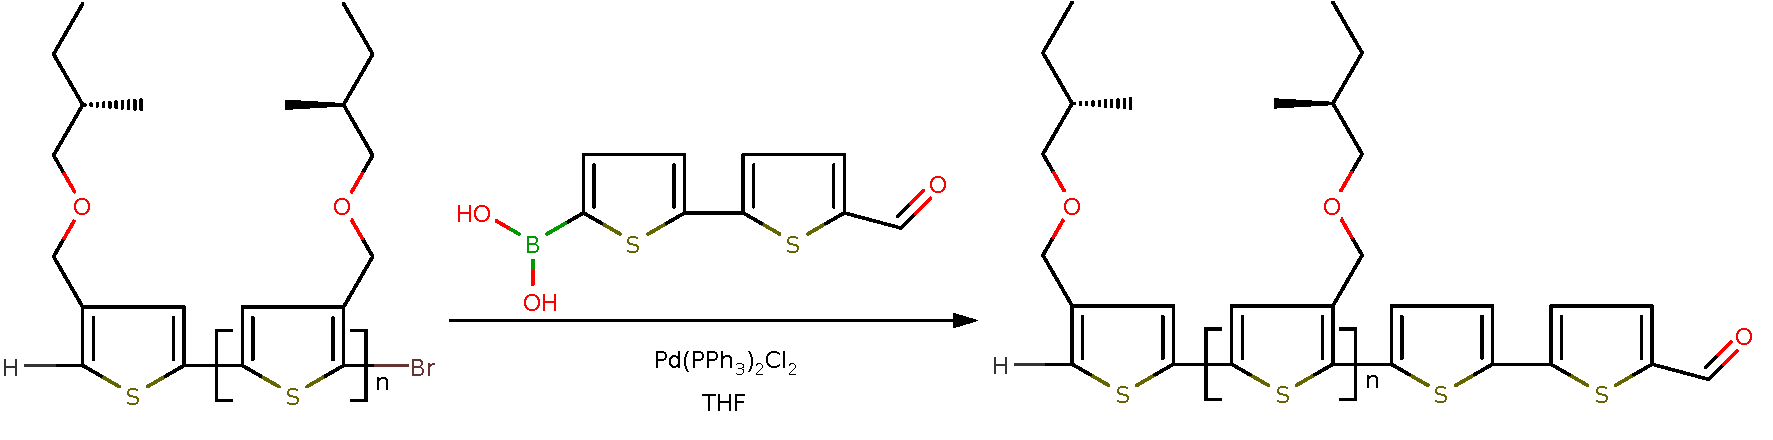
\includegraphics[scale=0.5]
{syn9-suzuki.pdf}
\end{figure}
Poly\{3-[((S)-2-methyl\-butyl\-oxy)\-methyl{]}\-thio\-phene\} \cmpd+{ig2-8} (\SI{14.4}{\mg}, quantity of chains estimated using $M_w$ \SI{0.976}{\umol}) was added in a \SI{100}{\mL} Schlenk tube with B-(5'-formyl[2,2'-bi\-thio\-phen]\-5-yl)\-boronic acid (\SI{1.37}{\mg}, \SI{5.75}{\umol}, solution in distilled tetrahydrofuran \SI{170}{\uL}) and bis(tri\-phenyl\-phosphine)\-palladium(II) dichloride (\ch{Pd(PPh3)2Cl2}, \SI{0.56}{\mg}, solution in distilled tetrahydrofuran \SI{175}{\uL}), then the mixture was dried on mechanical pump. 
Under nitrogen atmosphere dry tetrahydrofuran (\SI{6}{\mL}) was added. De\-oxy\-gen\-ated sodium carbonate aqueous solution (\SI{1}{\Molar}, \SI{1}{\mL}) was added and the reaction was refluxed for \SI{24}{\hour} under stirring in nitrogen atmosphere.
At room temperature the reaction was quenched by adding distilled water (\SI{10}{\mL}) and extracted with dichloromethane (3 $\times$ \SI{20}{\mL}). The collected organic fractions were washed with water, concentrated then poured in methanol (\SI{100}{\mL}). The precipitated was filtered (\gls{PTFE} membrane, \SI{0.45}{\um} porosity), washed with diethyl ether and solubilized again in chloroform. The chloroform solution was precipitated in methanol and filtered a second time obtaining a red solid \cmpd+{ig2-19} (\SI{11}{\mg}, 76~\% yield).

{\HNMR} (\SI{600}{\MHz}, \gls{TCE}-d$_2$) $\delta$ (ppm) 9.80 (s, 0.015H, \ch{H-C=O}), 7.21 (s, 1H, arom.\ H), 4.54 (s, 2H, \ch{CCH2O}), 3.40 (dd, $J =$ \SI{9.0}{\Hz} (geminal), \SI{6.1}{\Hz}, 1H, \ch{OC\underline{H}2CH}), 3.33 -- 3.29 (m, 1H, \ch{OC\underline{H}2CH}), 1.76 -- 1.65 (m, 1H, \ch{OCH2C\underline{H}}), 1.52 -- 1.40 (m, 1H, \ch{OCH2CHC\underline{H}2}), 1.20 -- 1.11 (m, 1H, \ch{OCH2CHC\underline{H}2}), 0.92 (d, $J =$ \SI{6.1}{\Hz}, 3H, \ch{CHC\underline{H}3}), 0.88 (t, $J =$ \SI{6.7}{\Hz}, 3H, \ch{CH2C\underline{H}3}).
\gls{FTIR} (film on \ch{KBr}) $\nu$ (\SI{}{\per\cm}) 2960, 2930, 2875, 1668, 1461, 1378, 1091, 840.

\subsection{Functionalization of Aldehyde on Polythiophene with Radical Polymerization Initiator (\cmpd+{ig2-22})}

\begin{figure}[H]%syn10-pt-tipno
\centering
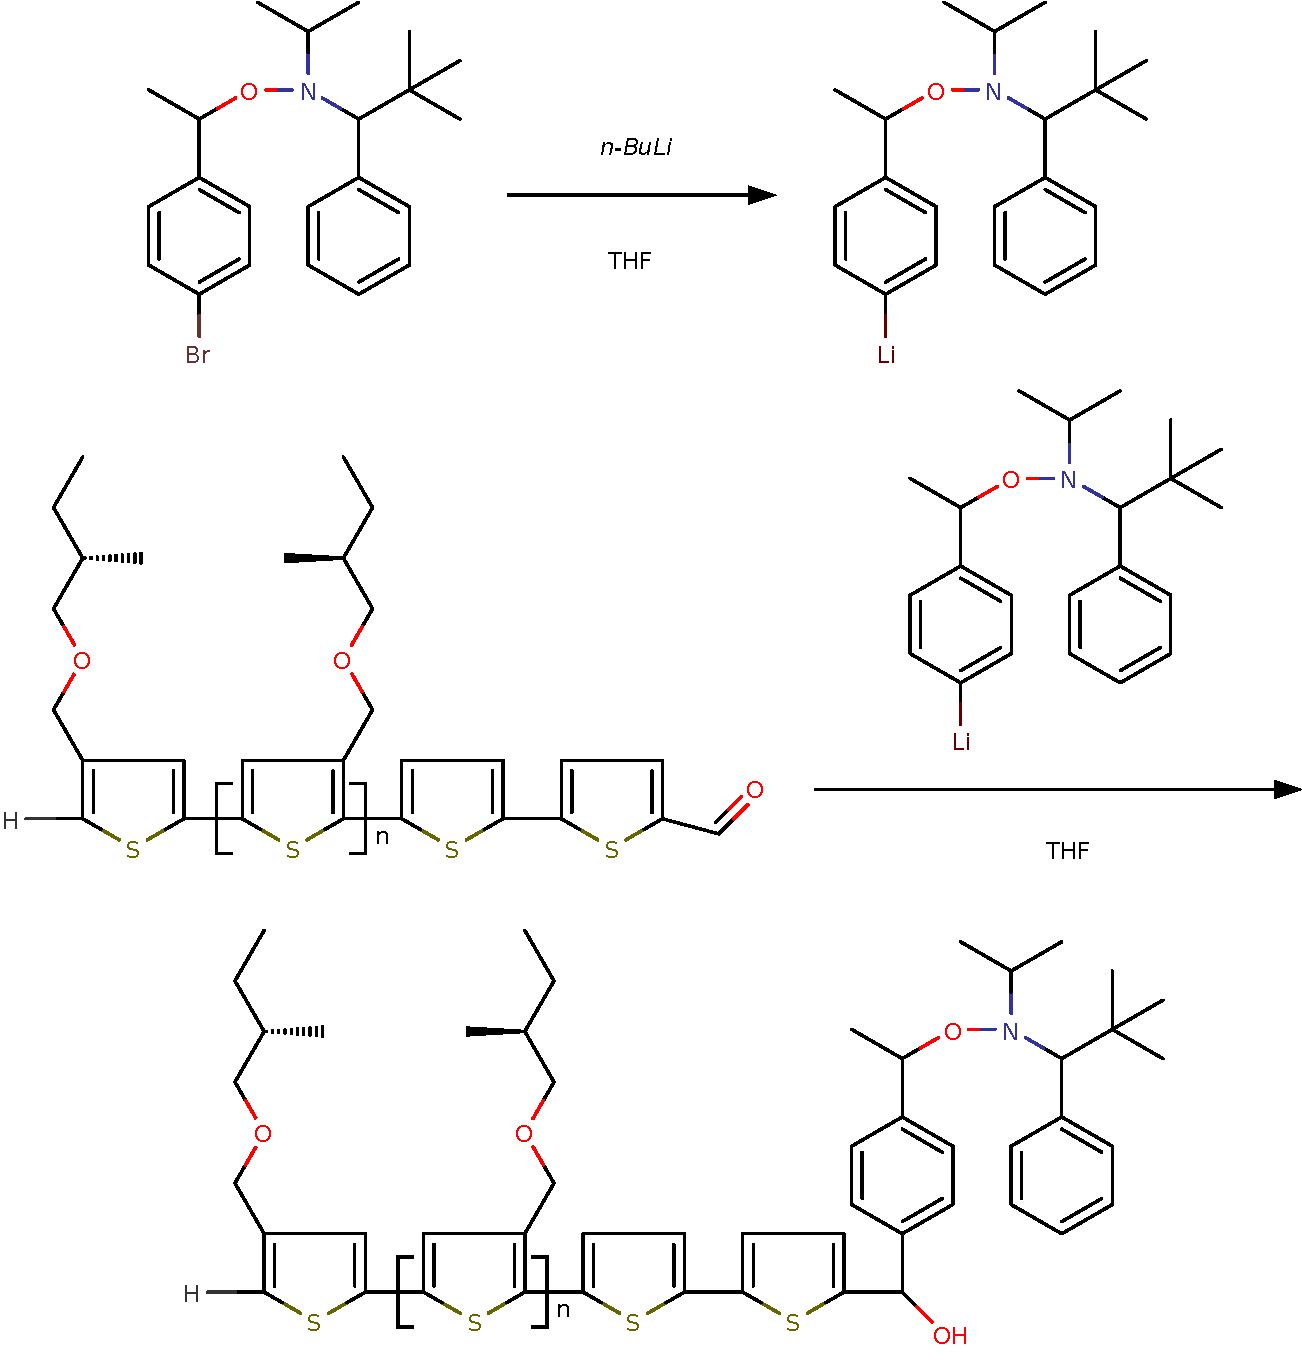
\includegraphics[scale=0.5]
{syn10-pt-tipno.pdf}
\end{figure}

The previously synthesized bromo-alkoxy\-amine \cmpd+{ig2-21} (\SI{33}{\mg}, mixture containing \SI{23}{\mg} of N-tert-butyl-O-[1-[4-bromo\-phenyl]\-ethyl]-N-(2-methyl-1-phenyl\-propyl)\-hydroxyl\-amine, \gls{BrPhEtTIPNO}, \SI{57}{\umol}; \SI{3}{\mg} of precursor \cmpd+{ig2-17}, \SI{11}{\umol}; \SI{7}{\mg} of dimerized precursor isomers \ch{(BrC6H4C2H4)2}, \SI{19}{\umol}) was dissolved in dry tetrahydrofuran (\SI{3}{\mL}) and cooled to \SI{-40}{\celsius}. 
A solution of \textit{n}-butyl\-lithium (\SI{1.6}{\Molar} in hexane, \SI{75}{\uL}, \SI{120}{\umol}) was added dropwise while stirring, then was allowed to warm to room temperature. In another flask polythiophene-aldehyde (\SI{10}{\mg}) was dried under vacuum and dissolved in dry tetrahydrofuran (\SI{3}{\mL}) at \SI{50}{\celsius}. 
The solution of lithiated alkoxy\-amine was transferred via syringe into a solution of polythiophene-aldehyde solution, the reaction was kept at \SI{50}{\celsius} for one hour, then at room temperature it was diluted with chloroform and poured in acetone (\SI{100}{\mL}). 
The red solid was collected by filtration (\gls{PTFE} membrane, \SI{0.45}{\um}), dissolved in chloroform and washed with methanol obtaining polythiophene-\gls{TIPNO} \cmpd+{ig2-22} as a red powder (\SI{9}{\mg}, yield $\approx90$~\%).

{\HNMR} (\SI{500}{\MHz}, \gls{TCE}-d$_2$) $\delta$ (ppm) 7.21 (s, 1H, arom.\ H), 4.54 (s, 2H, \ch{CCH2O}), 3.43 -- 3.36 (m, 1H, \ch{OC\underline{H}2CH}), 3.34 -- 3.27 (m, 1H, \ch{OC\underline{H}2CH}), 1.76 -- 1.64 (m, 2H, \ch{OCH2C\underline{H}}), 1.51 -- 1.42 (m, 1H, \ch{OCH2CHC\underline{H}2}), 1.19 -- 1.10 (m, 1H, \ch{OCH2CHC\underline{H}2}), 0.92 (d, $J =$ \SI{6.4}{\Hz}, 3H, \ch{CHC\underline{H}3}), 0.88 (t, $J =$ \SI{7.2}{\Hz}, 3H, \ch{CH2C\underline{H}3}).

\subsection[Poly\{3-[((S)-2-methyl\-butyl\-oxy)\-methyl{]}\-thio\-phene\}-\textit{block}-poly(4-vinyl\-pyridine) (\cmpd+{sz17})]{Poly\{3-[((S)-2-methyl\-butyl\-oxy)\-methyl{]}\-thio\-phene\}-\textit{block}-poly(4-vinyl\-pyridine) (\cmpd+{sz17}) \\ NMRP polymerization of 4-vinyl\-pyridine}

\begin{figure}[H]%syn11-p4vp
\centering
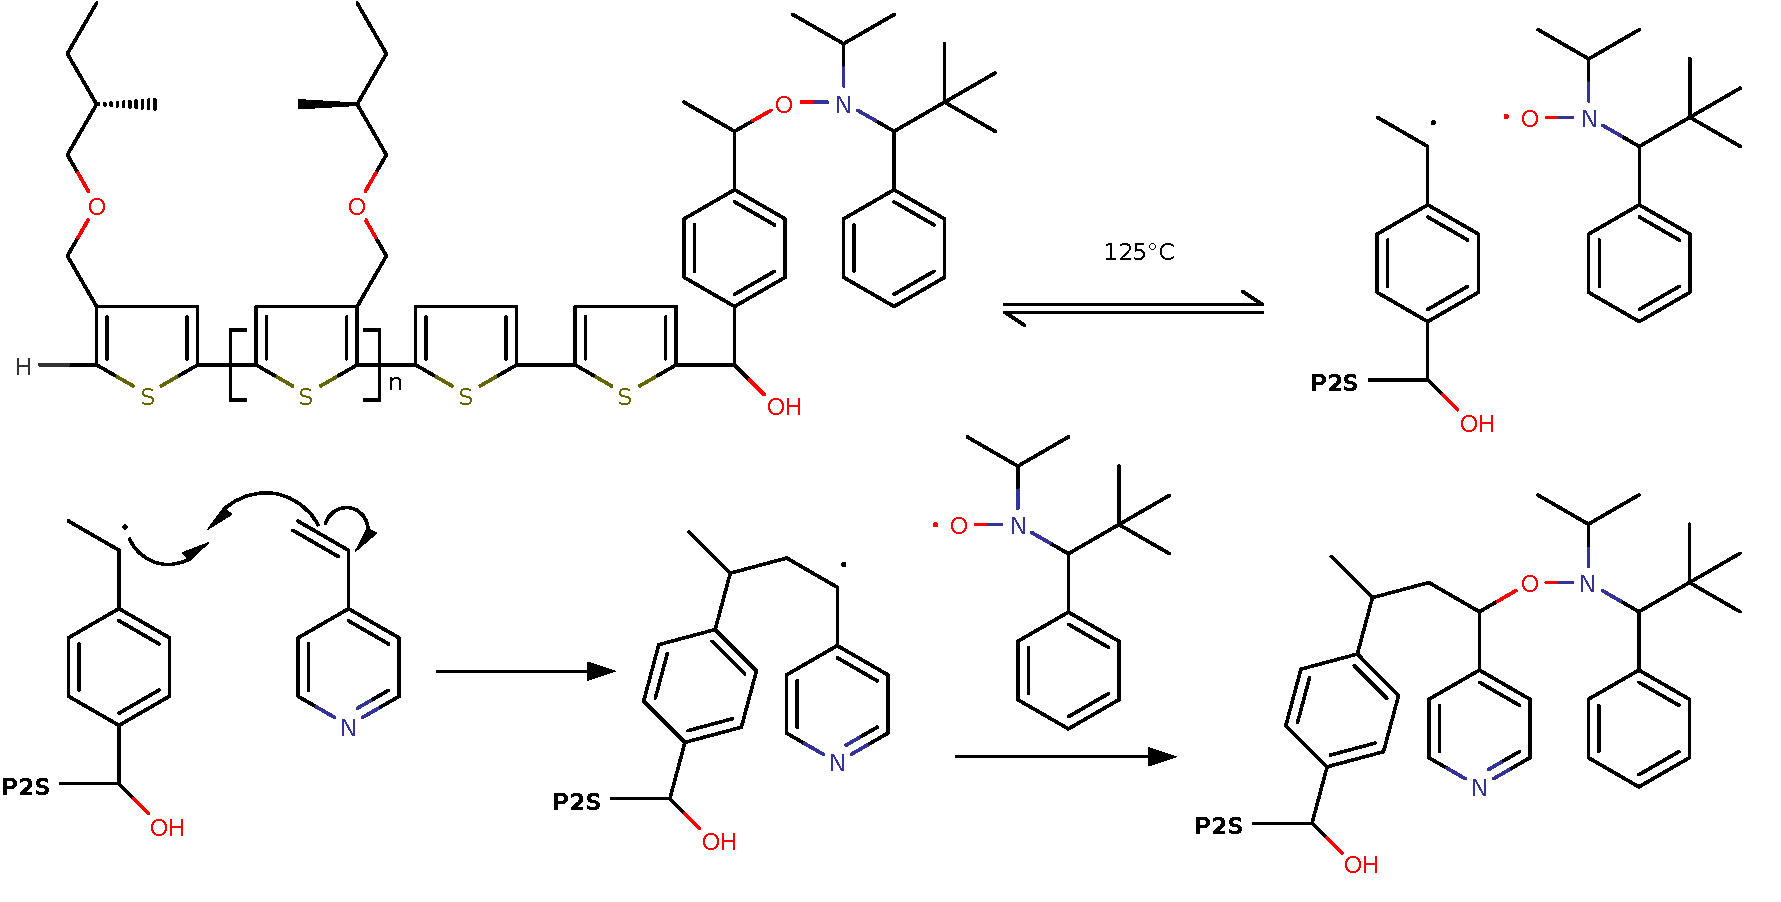
\includegraphics[scale=0.5]
{syn11-p4vp.pdf}
\end{figure}

Polythiophene-\gls{TIPNO} \cmpd+{ig2-22} (\SI{9}{\mg}, \SI{0.9}{\umol} of polymeric chains) in a Schlenk tube was dissolved in degassed ortho-di\-chloro\-benzene (\SI{2}{\mL}) and sonicated. Then 4-vinyl\-pyridine (\SI{291}{\uL}, \SI{2.7}{\mmol}) and \acrlong{TIPNO} (\gls{TIPNO} radical, \SI{10}{\uL} of a 1~\% solution in ortho-di\-chloro\-benzene, \SI{0.4}{\umol}) were added. The whole reaction mixture was passed through three freeze/pump/thaw cycles and heated to \SI{125}{\celsius}. 
After \SI{4}{\hour} the mixture showed no changes in color or viscosity and the reaction was stopped cooling in liquid nitrogen. Then at room temperature was diluted with chloroform (\SI{2}{\mL}), poured in hexane (\SI{400}{\mL}) and stirred overnight. 
The so-obtained solid product was filtered (\gls{PTFE} membrane, \SI{0.45}{\um}), recovered in chloroform and precipitated again in methanol. The orange solid was washed first with hot toluene (\SI{70}{\celsius}) and the remaining product was recovered with chloroform to achieve two different fractions (\SI{6}{\mg} in toluene and \SI{6}{\mg} in chloroform).

{\HNMR} (\SI{600}{\MHz}, \ch{CDCl3}) $\delta$ (ppm) 8.36 (broad s, \gls{P4VP} arom.\ near N), 7.24 (s, thiop.\ arom.\ H), 6.48 (broad s, \gls{P4VP} arom.\ far N), 4.58 (s, thioph.\ \ch{CCH2O}), 3.49 -- 3.40 (m, thioph.\ \ch{OC\underline{H}2CH}), 3.39 -- 3.29 (m, thioph.\ \ch{OC\underline{H}2CH}), 1.78 -- 1.69 (m, thioph.\ \ch{OCH2C\underline{H}}), 1.55 -- 1.49 (m, thioph.\ \ch{OCH2CHC\underline{H}2}), 0.97 (d, $J =$ \SI{6.3}{\Hz}, thioph.\ \ch{CHC\underline{H}3}), 0.92 (t, $J =$ \SI{7.5}{\Hz}, thioph.\ \ch{CH2C\underline{H}3}), 0.90 -- 0.83 (m, \gls{P4VP} aliph.).

{\HNMR} (\SI{600}{\MHz}, \gls{TCE}) $\delta$ (ppm) 8.26 (broad s, \gls{P4VP} arom.\ near N), 7.21 (s, thiop.\ arom.\ H), 6.35 (broad s, \gls{P4VP} arom.\ far N), 4.54 (s, thioph.\ \ch{CCH2O}), 3.44 -- 3.35 (m, thioph.\ \ch{OC\underline{H}2CH}), 3.34 -- 3.25 (m, thioph.\ \ch{OC\underline{H}2CH}), 1.73 -- 1.65 (m, thioph.\ \ch{OCH2C\underline{H}}), 1.57 -- 1.38 (m, thioph.\ \ch{OCH2CHC\underline{H}2}), 0.92 (d, $J =$ \SI{6.5}{\Hz}, thioph.\ \ch{CHC\underline{H}3}), 0.88 (t, $J =$ \SI{7.4}{\Hz}, thioph.\ \ch{CH2C\underline{H}3}), 0.85 -- 0.77 (m, H, \gls{P4VP} aliph.).
\end{section}